% =============================================================================
% optical_path.tex - Side-view optical path diagram for the beamsplitter
% headset architecture. Adapted from slides_latex/f7_main.tex with the
% following changes for use in chap_3_hardware.tex section 3.1.3:
%   - Display reduced to 35 mm width (halfW = 17.5) and 4.6 mm thickness
%   - Beamsplitter extended to 1.2x total length (bsHalfDiag = 19.2)
%   - Headset label moved inside the frame at top-left corner; leader removed
%   - Lens orientation kept (curved face toward the eye - the collimated side
%     for the dominant display->eye path; report section 3.2.1 prose
%     contradicts this and should be edited separately)
% =============================================================================
\documentclass[tikz,border=4mm]{standalone}

\usepackage[T1]{fontenc}
\usepackage{carlito}
\renewcommand{\familydefault}{\sfdefault}
\usepackage{tikz}
\usetikzlibrary{calc, positioning, arrows.meta, decorations.markings, fadings}

% --- Colours ---
\definecolor{visiblec}{HTML}{1F77B4}
\definecolor{nirc}{HTML}{C84E4E}
\definecolor{frameC}{HTML}{1F1F1F}
\definecolor{lensTint}{HTML}{B5D5E8}
\definecolor{lensStroke}{HTML}{6090A8}
\definecolor{glassTint}{HTML}{B0B5C0}
\definecolor{glassStroke}{HTML}{707880}
\definecolor{cameraC}{HTML}{3A3A3A}
\definecolor{displayC}{HTML}{2A2A2A}
\definecolor{displayEdge}{HTML}{606060}
\definecolor{eyeOutline}{HTML}{1F1F1F}
\definecolor{irisC}{HTML}{5C7C9A}
\definecolor{labelC}{HTML}{1F1F1F}

% --- Line-width palette ---
\def\lwFrame{2.5pt}
\def\lwVisible{1.2pt}
\def\lwIR{1.1pt}
\def\lwLens{1.0pt}
\def\lwDisplay{0.8pt}
\def\lwBS{2.8pt}
\def\lwEye{1.2pt}

% --- Geometry: headset frame ---
\def\headsetBackX{-45}
\def\headsetFrontX{100}
\def\headsetTopY{50}
\def\headsetBotY{-50}
\def\eyeOpeningTopY{18}
\def\eyeOpeningBotY{-18}

% --- Geometry: camera ---
\def\cameraCx{-30}
\def\cameraW{20}
\def\cameraH{10}
\def\cameraNubLen{4}
\def\cameraNubH{6}

% --- Geometry: beamsplitter (45 degrees, "\" orientation) ---
% MOD: bsHalfDiag 16 -> 19.2 (1.2x total length: 32 mm -> 38.4 mm)
\def\bsCx{30}
\def\bsCy{0}
\def\bsHalfDiag{19.2}

% --- Geometry: display ---
% MOD: halfW 39 -> 17.5 (35 mm full width); thickness 9.2 mm -> 4.6 mm
\def\displayCx{30}
\def\displayBotY{22}
\def\displayTopY{26.6}
\def\displayHalfW{17.5}

% --- Geometry: plano-convex lens (flat -> beamsplitter, curved -> eye) ---
\def\lensX{75}
\def\lensHalfH{15}
\def\lensBulge{6}

% --- Geometry: IR LED ring ---
\def\irRingX{97.8}
\def\irRingY{15.5}
\def\irLEDr{2.2}

% --- Geometry: eye ---
\def\eyeX{125}
\def\eyeR{12}
\def\pupilOffset{5}
\def\irisR{5}
\def\pupilR{2}

\begin{document}
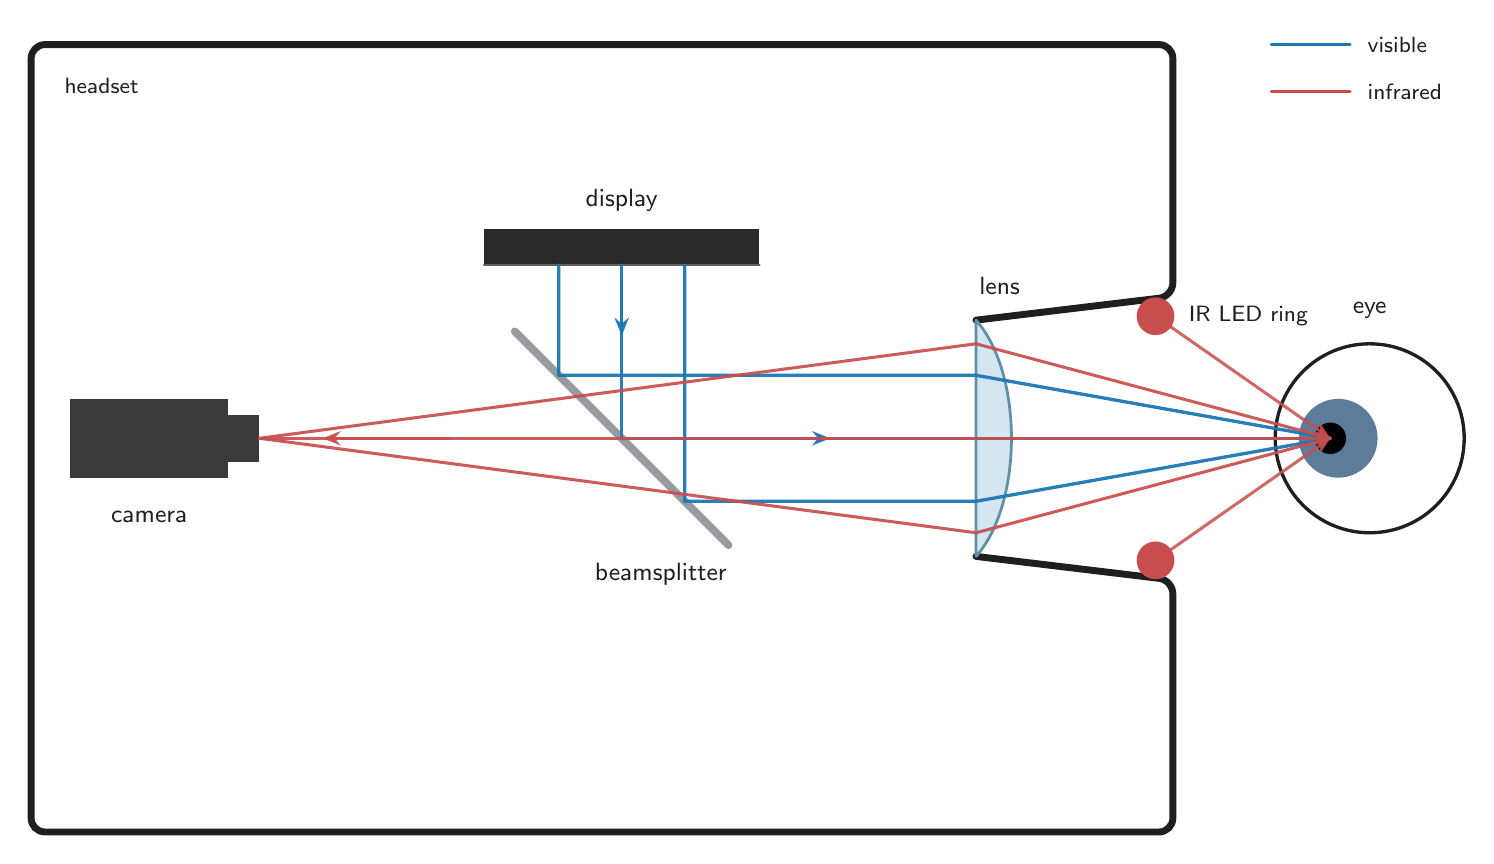
\begin{tikzpicture}[x=1mm, y=1mm, line cap=round, line join=round, font=\sffamily]

  \pgfmathsetmacro{\pupilXcoord}{\eyeX-\pupilOffset}
  \pgfmathsetmacro{\camNubFront}{\cameraCx+\cameraW/2+\cameraNubLen}
  \pgfmathsetmacro{\bsHalfProj}{\bsHalfDiag/sqrt(2)}
  \pgfmathsetmacro{\bsTLx}{\bsCx-\bsHalfProj}
  \pgfmathsetmacro{\bsTLy}{\bsCy+\bsHalfProj}
  \pgfmathsetmacro{\bsBRx}{\bsCx+\bsHalfProj}
  \pgfmathsetmacro{\bsBRy}{\bsCy-\bsHalfProj}

  % Headset frame
  \draw[frameC, line width=\lwFrame, rounded corners=5]
    (\lensX, \lensHalfH)
    -- (\headsetFrontX, \eyeOpeningTopY)
    -- (\headsetFrontX, \headsetTopY)
    -- (\headsetBackX,  \headsetTopY)
    -- (\headsetBackX,  \headsetBotY)
    -- (\headsetFrontX, \headsetBotY)
    -- (\headsetFrontX, \eyeOpeningBotY)
    -- (\lensX, -\lensHalfH);

  % MOD: Headset label moved inside the frame at top-left, no leader line
  \node[labelC, anchor=north west, font=\sffamily\footnotesize]
    at ({\headsetBackX + 3}, {\headsetTopY - 3}) {headset};

  % Camera
  \fill[cameraC]
    ({\cameraCx-\cameraW/2}, {-\cameraH/2}) rectangle ({\cameraCx+\cameraW/2}, {\cameraH/2});
  \fill[cameraC]
    ({\cameraCx+\cameraW/2}, {-\cameraNubH/2}) rectangle ({\cameraCx+\cameraW/2+\cameraNubLen}, {\cameraNubH/2});

  % Display
  \fill[displayC]
    ({\displayCx-\displayHalfW}, \displayBotY) rectangle ({\displayCx+\displayHalfW}, \displayTopY);
  \draw[displayEdge, line width=\lwDisplay]
    ({\displayCx-\displayHalfW}, \displayBotY) -- ({\displayCx+\displayHalfW}, \displayBotY);

  % Beamsplitter
  \draw[glassStroke, line width=\lwBS, opacity=0.75]
    (\bsTLx, \bsTLy) -- (\bsBRx, \bsBRy);

  % Plano-convex lens: flat side at lensX, convex bulging right toward eye
  \draw[line width=\lwLens, fill=lensTint!60, draw=lensStroke]
    (\lensX, {-\lensHalfH}) -- (\lensX, {\lensHalfH})
    .. controls ({\lensX+\lensBulge}, {\lensHalfH*0.55}) and ({\lensX+\lensBulge}, {-\lensHalfH*0.55})
    .. (\lensX, {-\lensHalfH});

  % IR LED ring (top + bottom stubs at the diagonal-vertical corner)
  \fill[nirc] (\irRingX,  \irRingY) circle (\irLEDr);
  \fill[nirc] (\irRingX, -\irRingY) circle (\irLEDr);
  \draw[nirc, line width=\lwIR] (\irRingX,  \irRingY) circle (\irLEDr);
  \draw[nirc, line width=\lwIR] (\irRingX, -\irRingY) circle (\irLEDr);

  % Eye
  \draw[eyeOutline, line width=\lwEye, fill=white]
    (\eyeX, 0) circle (\eyeR);
  \fill[irisC]   ({\eyeX-\pupilOffset+1}, 0) circle (\irisR);
  \fill[black]   ({\eyeX-\pupilOffset}, 0) circle (\pupilR);

  % --- VISIBLE rays: display down -> bs reflect -> lens -> eye ---
  \draw[visiblec, line width=\lwVisible, opacity=0.95]
    ({\displayCx-8}, \displayBotY) -- ({\displayCx-8}, 8) -- (\lensX, 8) -- (\pupilXcoord, 0);
  \draw[visiblec, line width=\lwVisible, opacity=0.95]
    (\displayCx, \displayBotY) -- (\displayCx, 0) -- (\lensX, 0) -- (\pupilXcoord, 0);
  \draw[visiblec, line width=\lwVisible, opacity=0.95]
    ({\displayCx+8}, \displayBotY) -- ({\displayCx+8}, -8) -- (\lensX, -8) -- (\pupilXcoord, 0);
  \draw[visiblec, -{Stealth[length=2.3mm, width=1.8mm]}, line width=\lwVisible, opacity=0.95]
    (\displayCx, {\displayBotY - 2}) -- (\displayCx, {\displayBotY/2 + 2});
  \draw[visiblec, -{Stealth[length=2.3mm, width=1.8mm]}, line width=\lwVisible, opacity=0.95]
    ({\bsCx + 6}, 0) -- ({(\bsCx + \lensX)/2 + 4}, 0);

  % --- IR illumination: LED stubs -> eye pupil (arrows indicate light direction) ---
  \draw[nirc, -{Stealth[length=2.3mm, width=1.8mm]}, line width=\lwIR, opacity=0.85]
    (\irRingX,  \irRingY) -- (\pupilXcoord, 0);
  \draw[nirc, -{Stealth[length=2.3mm, width=1.8mm]}, line width=\lwIR, opacity=0.85]
    (\irRingX, -\irRingY) -- (\pupilXcoord, 0);

  % --- NIR imaging return: pupil -> lens -> through bs -> camera ---
  \draw[nirc, line width=\lwIR, opacity=0.92]
    (\pupilXcoord, 0) -- (\lensX, 12) -- (\camNubFront, 0);
  \draw[nirc, line width=\lwIR, opacity=0.92]
    (\pupilXcoord, 0) -- (\lensX,  0) -- (\camNubFront, 0);
  \draw[nirc, line width=\lwIR, opacity=0.92]
    (\pupilXcoord, 0) -- (\lensX, -12) -- (\camNubFront, 0);
  \draw[nirc, -{Stealth[length=2.3mm, width=1.8mm]}, line width=\lwIR, opacity=0.92]
    ({(\bsCx+\cameraCx)/2 + 8}, 0) -- ({(\bsCx+\cameraCx)/2 - 8}, 0);

  % Labels
  \node[labelC, anchor=north, font=\sffamily\small] at (\cameraCx, {-\cameraH/2 - 3}) {camera};
  \node[labelC, anchor=south, font=\sffamily\small] at (\displayCx, {\displayTopY + 1}) {display};
  \node[labelC, anchor=north east, font=\sffamily\small]
    at ({\bsBRx + 1}, {\bsBRy - 1}) {beamsplitter};
  \node[labelC, anchor=south, font=\sffamily\small] at ({\lensX+\lensBulge/2}, {\lensHalfH + 2}) {lens};
  \node[labelC, anchor=west, font=\sffamily\footnotesize] at ({\irRingX + 3}, {\irRingY}) {IR LED ring};
  \node[labelC, anchor=south, font=\sffamily\small] at (\eyeX, {\eyeR + 2}) {eye};

  % Legend (top-right, above the eye, top in line with the headset frame top)
  \begin{scope}[shift={(112.5, 44)}]
    \draw[visiblec, line width=\lwVisible] (0, 6) -- (10, 6);
    \node[labelC, anchor=west, font=\sffamily\footnotesize] at (11, 6) {visible};
    \draw[nirc, line width=\lwIR] (0, 0) -- (10, 0);
    \node[labelC, anchor=west, font=\sffamily\footnotesize] at (11, 0) {infrared};
  \end{scope}
\end{tikzpicture}
\end{document}
